\section{Implementation}
För att genomföra projektet så användes följande:
\begin{itemize}
\item C++ som programmeringsspråk fast en del bibliotek var skrivna i C
\item Objektorienterad kod
\item OpenGL för alla 3D effekter
\item X11 biblioteket för textöverläggning
\item OpenCV för inläsning av alla bilder och konvertering till ett format som OpenGl kunde använda
\item Boost::Filesystem för tillgång till datorns filsystem
\item MicroGlut för fönster och händelser hantering i OpenGL applikationen
\item VectorUtils3 för vektor och matrisoperationer
\item make för att snabbt kunna bygga hela programmet
\item Git för versionshantering
\item Eclipse som utvecklingsmiljö
\end{itemize}
\begin{center}
\begin{figure}[H]
    \centering
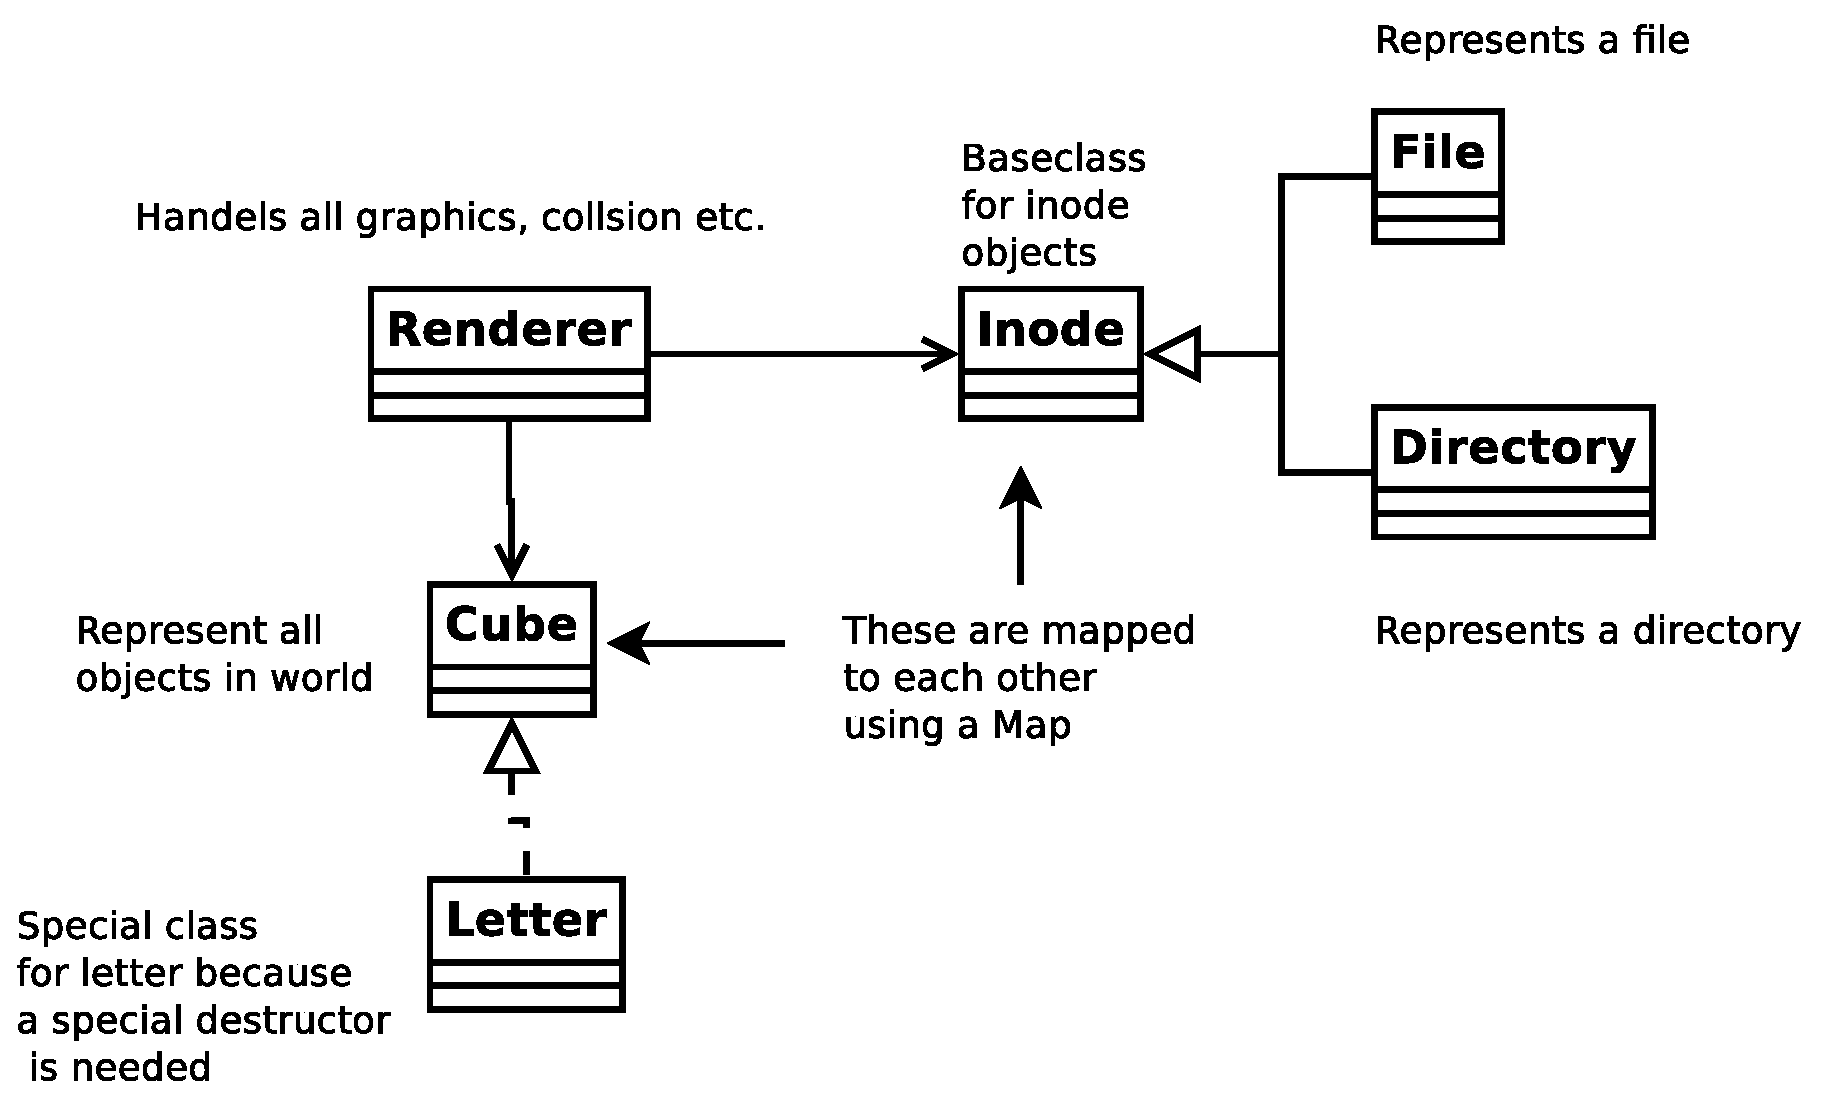
\includegraphics[width=10cm]{../grafik/uml.eps}
\caption{TMBTRF UML.}
\label{fig:uml}
\end{figure}
\end{center}
I figur~\ref{fig:uml} kan man se den grundläggande strukturen över programmet. Den är lite mer invecklad i verkligheten men den ger en bra överblick. När programmet startar så skapas först en Directory instans som representerar den mappen man startar programmet ifrån. Klassen Directory innehåller en Vector av Inodes objekt som representerar alla filer och mappar som ligger i den nuvarande mappen. Efter att denna vektor har initierats så skickas denna Directory instant in i en konstruktor för Renderer som skapar en Renderer instant med inititerar OpenGL applikationen med hjälp av MicroGlut. I konstruktorn så inititeras även en Vector i klassen som innehåller en massa Cube objekt som representerer golvet, skydomen och även alla filer och mappar. 
Om en Cube instans representerar ett Inode objekt så mappas dessa mot varandra med hjälp av en Map.
\\
\\
I början var även alla bokstäver ovanför alla Inodes objekt Cubes. Problemet med detta var att destruktorn för Cube raderar Model i klassen och eftersom alla bokstäver använder samma Model så blev alla bokstäver en Letter klass med en egen destruktorn som ej är virtuell så Cubes destruktor kallas ej på från Letters destruktor.
\\
\\
När alla Cube objekt har generetars så startar GLUTs loop och den kallar på Renderers display funktionen som i princip endast går igenom alla Cube objekt och kallar på varje objekts egna display funktion. Detta gör denna implementationen väldigt allmän och det är lätt att implementera nya objekt i världen. Till exempel så la jag till så jag kunde dra linjer i 3d världen vilket först endast var för att testa om pickingen fungerade som den skulle men sedan såg det rätt coolt ut så jag lät det vara kvar. Att implementera detta var väldigt lätt och krävde endast en ny funktion som genererade ett Cube objekt och en special display funktion för linjer. Renderers display funktion gör lite andra saker också såsom att kolla efter kollisioner och kolla om något objekt ska tas bort såsom linjer som endast existerar i 5 sekunder.

\subsection{Terminalen}
De kommandona som är implementerade är:
\begin{itemize}
\item select filename : som väljer en mapp/fil precis som om du skulle klicka på den 
\item help : som visar alla tillgängliga kommandon
\item cd directory : som gör att du går in i mappen precis som om du skulle gå in i den i världen
\item  rename filename new\_filename : som byter namn på filen
\item delete filename : som raderar filen
\end{itemize}
I cd, rename och delete kan du också skriva active istället för filnamnet så används den filen/mappen du har klickat på eller valt med select.

\subsection{Bygga programmet}
Skulle du vilja bygga programmet så måste det göras på en Linux dator med Microglut och Vectorutils3 i lib mappen för jag har modifierat båda med lite nya funktioner. Sedan behövs minst g++ version 4.9 för jag använder regex iterator som kom först i den versionen.